\documentclass[12pt]{article}
%NOTE: This report format is 

\newcommand{\reporttitle}{Rapport de Projet : Régulation d’un bâtiment thermiquement actif}
\newcommand{\reportauthorOne}{Benjamin BOCK}
\newcommand{\cidOne}{s2304467}
\newcommand{\reportauthorTwo}{Odayfa DAKIR}
\newcommand{\cidTwo}{s2305341}
\newcommand{\reportauthorThree}{Yazan SALOUM}
\newcommand{\cidThree}{s2304645}
\newcommand{\reporttype}{Coursework}
\bibliographystyle{plain}

% include files that load packages and define macros
\usepackage{fontspec}
\usepackage{newtxtext,newtxmath} % Times New Roman pour texte et maths



% Packages utiles (ajoutez ceux dont vous avez besoin)
\usepackage[letterpaper,hmargin=2.8cm,vmargin=2.0cm,includeheadfoot]{geometry}
\usepackage{textpos}
\usepackage{natbib}
\usepackage{stackengine}
\usepackage{tabularx,longtable,multirow,subfigure,caption}%hangcaption
\usepackage{fncylab} %formatting of labels
\usepackage{fancyhdr}
\usepackage{color}
\usepackage[tight,ugly]{units}
\usepackage{url}
\usepackage{float}
\usepackage[english]{babel}
\usepackage{amsmath}
\usepackage{graphicx}
\usepackage[colorinlistoftodos]{todonotes}
\usepackage{dsfont}
\usepackage{epstopdf} % automatically replace .eps with .pdf in graphics
\usepackage{backref}
\usepackage{array}
\usepackage{etoolbox}
\usepackage{enumerate} % for numbering with [a)] format 
\usepackage{tcolorbox}
\usepackage{graphicx} % Pour insérer des images
\usepackage{tocloft}  % Pour personnaliser la liste des figures


% table of content
\renewcommand{\tableofcontentsname}{Table of Contents}

% table of figures
\renewcommand{\listfigurename}{Table of Figures}

% various theorems
\usepackage{ntheorem}
\theoremstyle{break}
\newtheorem{lemma}{Lemma}
\newtheorem{theorem}{Theorem}
\newtheorem{remark}{Remark}
\newtheorem{definition}{Definition}
\newtheorem{proof}{Proof}

% example-environment
\newenvironment{example}[1][]
{ 
\vspace{4mm}
\noindent\makebox[\linewidth]{\rule{\hsize}{1.5pt}}
\textbf{Example #1}\\
}
{ 
\noindent\newline\makebox[\linewidth]{\rule{\hsize}{1.0pt}}
}

\setlength{\parindent}{0em}  % indentation of paragraph

\setlength{\headheight}{14.5pt}
\pagestyle{fancy}
\fancyfoot[ER,OR]{\thepage}%Page no. in the left on
                                %odd pages and on right on even pages
\fancyfoot[OC,EC]{\sffamily }
\renewcommand{\headrulewidth}{0.1pt}
\renewcommand{\footrulewidth}{0.1pt}
\captionsetup{margin=10pt,font=small,labelfont=bf}

%--- chapter heading
\def\@makechapterhead#1{%
  \vspace*{10\p@}%
  {\parindent \z@ \raggedright
    \interlinepenalty\@M
    \Huge \bfseries 
    \thechapter \space\space #1\par\nobreak
    \vskip 30\p@
  }}

%---chapter heading for \chapter*  
\def\@makeschapterhead#1{%
  \vspace*{10\p@}%
  {\parindent \z@ \raggedright
    \interlinepenalty\@M
    \Huge \bfseries  
    #1\par\nobreak
    \vskip 30\p@
  }}

% %%%%%%%%%%%%% boxit
\def\Beginboxit
   {\par
    \vbox\bgroup
	   \hrule
	   \hbox\bgroup
		  \vrule \kern1.2pt %
		  \vbox\bgroup\kern1.2pt
   }

\def\Endboxit{%
			      \kern1.2pt
		       \egroup
		  \kern1.2pt\vrule
		\egroup
	   \hrule
	 \egroup
   }	

\newenvironment{boxit}{\Beginboxit}{\Endboxit}
\newenvironment{boxit*}{\Beginboxit\hbox to\hsize{}}{\Endboxit}

\allowdisplaybreaks

\makeatletter
\newcounter{elimination@steps}
\newcolumntype{R}[1]{>{\raggedleft\arraybackslash$}p{#1}<{$}}
\def\elimination@num@rights{}
\def\elimination@num@variables{}
\def\elimination@col@width{}
\newenvironment{elimination}[4][0]
{
    \setcounter{elimination@steps}{0}
    \def\elimination@num@rights{#1}
    \def\elimination@num@variables{#2}
    \def\elimination@col@width{#3}
    \renewcommand{\arraystretch}{#4}
    \start@align\@ne\st@rredtrue\m@ne
}
{
    \endalign
    \ignorespacesafterend
}
\newcommand{\eliminationstep}[2]
{
    \ifnum\value{elimination@steps}>0\leadsto\quad\fi
    \left[
        \ifnum\elimination@num@rights>0
            \begin{array}
            {@{}*{\elimination@num@variables}{R{\elimination@col@width}}
            |@{}*{\elimination@num@rights}{R{\elimination@col@width}}}
        \else
            \begin{array}
            {@{}*{\elimination@num@variables}{R{\elimination@col@width}}}
        \fi
            #1
        \end{array}
    \right]
    & 
    \begin{array}{l}
        #2
    \end{array}
    &%                                    moved second & here
    \addtocounter{elimination@steps}{1}
}
\makeatother

%% Fast macro for column vectors
\makeatletter  
\def\colvec#1{\expandafter\colvec@i#1,,,,,,,,,\@nil}
\def\colvec@i#1,#2,#3,#4,#5,#6,#7,#8,#9\@nil{% 
  \ifx$#2$ \begin{bmatrix}#1\end{bmatrix} \else
    \ifx$#3$ \begin{bmatrix}#1\\#2\end{bmatrix} \else
      \ifx$#4$ \begin{bmatrix}#1\\#2\\#3\end{bmatrix}\else
        \ifx$#5$ \begin{bmatrix}#1\\#2\\#3\\#4\end{bmatrix}\else
          \ifx$#6$ \begin{bmatrix}#1\\#2\\#3\\#4\\#5\end{bmatrix}\else
            \ifx$#7$ \begin{bmatrix}#1\\#2\\#3\\#4\\#5\\#6\end{bmatrix}\else
              \ifx$#8$ \begin{bmatrix}#1\\#2\\#3\\#4\\#5\\#6\\#7\end{bmatrix}\else
                 \PackageError{Column Vector}{The vector you tried to write is too big, use bmatrix instead}{Try using the bmatrix environment}
              \fi
            \fi
          \fi
        \fi
      \fi
    \fi
  \fi 
}  
\makeatother

\robustify{\colvec} % various packages needed for maths etc.
% quick way of adding a figure
\newcommand{\fig}[3]{
 \begin{center}
 \scalebox{#3}{\includegraphics[#2]{#1}}
 \end{center}
}

%\newcommand*{\point}[1]{\vec{\mkern0mu#1}}
\newcommand{\ci}[0]{\perp\!\!\!\!\!\perp} % conditional independence
\newcommand{\point}[1]{{#1}} % points 
\renewcommand{\vec}[1]{{\boldsymbol{{#1}}}} % vector
\newcommand{\mat}[1]{{\boldsymbol{{#1}}}} % matrix
\newcommand{\R}[0]{\mathds{R}} % real numbers
\newcommand{\Z}[0]{\mathds{Z}} % integers
\newcommand{\N}[0]{\mathds{N}} % natural numbers
\newcommand{\nat}[0]{\mathds{N}} % natural numbers
\newcommand{\Q}[0]{\mathds{Q}} % rational numbers
\ifxetex
\newcommand{\C}[0]{\mathds{C}} % complex numbers
\else
\newcommand{\C}[0]{\mathds{C}} % complex numbers
\fi
\newcommand{\tr}[0]{\text{tr}} % trace
\renewcommand{\d}[0]{\mathrm{d}} % total derivative
\newcommand{\inv}{^{-1}} % inverse
\newcommand{\id}{\mathrm{id}} % identity mapping
\renewcommand{\dim}{\mathrm{dim}} % dimension
\newcommand{\rank}[0]{\mathrm{rk}} % rank
\newcommand{\determ}[1]{\mathrm{det}(#1)} % determinant
\newcommand{\scp}[2]{\langle #1 , #2 \rangle}
\newcommand{\kernel}[0]{\mathrm{ker}} % kernel/nullspace
\newcommand{\img}[0]{\mathrm{Im}} % image
\newcommand{\idx}[1]{{(#1)}}
\DeclareMathOperator*{\diag}{diag}
\newcommand{\E}{\mathds{E}} % expectation
\newcommand{\var}{\mathds{V}} % variance
\newcommand{\gauss}[2]{\mathcal{N}\big(#1,\,#2\big)} % gaussian distribution N(.,.)
\newcommand{\gaussx}[3]{\mathcal{N}\big(#1\,|\,#2,\,#3\big)} % gaussian distribution N(.|.,.)
\newcommand{\gaussBig}[2]{\mathcal{N}\left(#1,\,#2\right)} % see above, but with brackets that adjust to the height of the arguments
\newcommand{\gaussxBig}[3]{\mathcal{N}\left(#1\,|\,#2,\,#3\right)} % see above, but with brackets that adjust to the height of the arguments
\DeclareMathOperator{\cov}{Cov} % covariance (matrix) 
\ifxetex
\renewcommand{\T}[0]{^\top} % transpose
\else
\newcommand{\T}[0]{^\top}
\fi
% matrix determinant
\newcommand{\matdet}[1]{
\left|
\begin{matrix}
#1
\end{matrix}
\right|
}



%%% various color definitions
\definecolor{darkgreen}{rgb}{0,0.6,0}

\newcommand{\blue}[1]{{\color{blue}#1}}
\newcommand{\red}[1]{{\color{red}#1}}
\newcommand{\green}[1]{{\color{darkgreen}#1}}
\newcommand{\orange}[1]{{\color{orange}#1}}
\newcommand{\magenta}[1]{{\color{magenta}#1}}
\newcommand{\cyan}[1]{{\color{cyan}#1}}


% redefine emph
\renewcommand{\emph}[1]{\blue{\bf{#1}}}

% place a colored box around a character
\gdef\colchar#1#2{%
  \tikz[baseline]{%
  \node[anchor=base,inner sep=2pt,outer sep=0pt,fill = #2!20] {#1};
    }%
}%
 % short-hand notation and macros


%%%%%%%%%%%%%%%%%%%%%%%%%%%%

\begin{document}
\sloppy % Permet plus de tolérance d'espace entre les mots

% front page
% Last modification: 2016-09-29 (Marc Deisenroth)
% Modification for UW: 2017-05-22 (jphickey)
\begin{titlepage}

\newcommand{\HRule}{\rule{\linewidth}{0.5mm}} % Defines a new command for the horizontal lines, change thickness here


%----------------------------------------------------------------------------------------
%	LOGO SECTION
%----------------------------------------------------------------------------------------



\begin{center} % Center remainder of the page

%----------------------------------------------------------------------------------------
%	HEADING SECTIONS
%----------------------------------------------------------------------------------------


\includegraphics[width = 15cm]{./figures/uliege_faculte_sciencesappliquees_logo_rvb}\\[1.5cm] 
\textbf{\textsc{\Large PROJ0001-1 Introduction \\
aux méthodes numériques et projet}}\\[1.0cm] 
\textsc{\Large Université de Liège}\\[0.5cm] 
\textsc{\large Faculté des Sciences Appliquées}\\[0.45cm] 
\textsc{\large Année académique 2024-2025}\\[0.45cm] 


%----------------------------------------------------------------------------------------
%	TITLE SECTION
%----------------------------------------------------------------------------------------

\HRule \\[0.4cm]
{ \huge \bfseries \reporttitle}\\ % Title of your document
\HRule \\[1.5cm]
\end{center}
%----------------------------------------------------------------------------------------
%	AUTHOR SECTION
%----------------------------------------------------------------------------------------

%\begin{minipage}{0.4\hsize}

\begin{center}
    \begin{minipage}{0.45\linewidth} % Bloc à gauche
        \raggedright % Aligné à gauche
        \normalsize \textit{Professeurs:} \\
            \small  Olivier BRULS \\
                    Quentin LOUVEAUX \\
                    Frédéric NGUYEN 
    \end{minipage}
    \begin{minipage}{0.45\linewidth} % Bloc à droite
        \raggedleft % Aligné à droite
        \normalsize \textit{Auteurs:} \\
        \begin{small}
            \reportauthorOne~(\cidOne)\\
            \reportauthorTwo~(\cidTwo)\\
            \reportauthorThree~(\cidThree)\\
        \end{small}
    \end{minipage}
\end{center}


\vspace{4cm}
\makeatletter
Liège, le \today

\vfill % Fill the rest of the page with whitespace



\makeatother

\end{titlepage}




%%%%%%%%%%%%%%%%%%%%%%%%%%% table of content
%If a table of content is needed, simply uncomment the following lines
\renewcommand{\contentsname}{Table des matières}
\renewcommand{\listfigurename}{Table des figures}
\renewcommand{\listtablename}{Liste des tableaux}

\tableofcontents
\listoffigures
\listoftables
\newpage


%%%%%%%%%%%%%%%%%%%%%%%%%%%% Main document
\section{Recherche de racines}

    Cette première question vise à modéliser deux fonctions : \texttt{secante(f,x0,x1,tol)} et \texttt{bissection(f,x0,x1,tol)}. Ces fonctions jouent le même rôle, qui est de rechercher la racine d'une fonction $f(x)$ donnée, mais ont des fonctionnements différents. Ainsi, selon le cas, c'est à l'étudiant à choisir, judicieusement, laquelle des deux se voit être la plus encline à être utilisée dans le contexte rencontré. Ces fonctions doivent retourner un objet de type \textit{list} avec deux valeurs, \texttt{x} et \texttt{statut}.
    
    \subsection{Bissection}
            La fonction \texttt{bissection} se base sur la méthode d'analyse numérique éponyme de recherche de racine. Celle-ci prend en arguments la fonction $f(x)$ elle-même, deux points d'abscisses différents et la tolérance d'erreur maximale admissible par l'algorithme. Afin d'assurer le bon fonctionnement de l'algorithme, il vient de vérifier les points suivants :
            \begin{enumerate}[label=\roman*.]
            \item Hypothèses de la méthode : 
                \begin{itemize}
                    \item 
                        Les images des deux points initiaux, \texttt{x0} et \texttt{x1}, doivent être de signes contraires. Ceci peut-être vérifié en testant le signe de l'expression $f(x_1)f(x_0)$. Ainsi, viennent deux cas possibles :
                        
                        \begin{itemize}
                            \item Cas 1, $f(x_1)f(x_0) < 0$ : \vspace{2mm} \\ 
                            Les deux images sont de signes contraires, l'hypothèse est donc vérifiée. \vspace{2mm} 
                            \item Cas 2, $f(x_1)f(x_0) > 0$ : \vspace{2mm} \\
                            Les deux images sont de mêmes signes, la méthode de la bissection n'est pas possible sur l'intervalle considéré. On retourne \texttt{statut = 1}.
                        \end{itemize}
                    \item
                        La fonction $f(x)$ doit être continue dans l'intervalle $[x_0 , x_1]$, soit $f \in C_0([x_0,x1])$. Malheureusement, aucune fonction de la bibliothèque standard Python ne le permet, tout comme les bibliothèques externes \texttt{numpy}, \texttt{scipy} et \texttt{matplotlib}. Il est ainsi impossible de prévoir le caractère de la fonction sur l'intervalle considéré. Supposons pour le projet que la fonction $f(x)$ dont on cherche la racine est bien continue sur l'intervalle. Nous verrons par la suite que cette hypothèse est acceptable car nous étudions un phénomène physique d'évolution de température dans un espace, en trois dimensions, continu, de sorte que la fonction est bien continue sur l'intervalle et l'hypothèse est vérifiée.
        
                \end{itemize}
            
            \item 
            Nombre d'appels de la fonction $f(x)$ :
                \begin{itemize}
                    \item Une attention particulière a été portée à ce sujet. En effet, l'algorithme n'appelle qu'une seule fois $f(x)$ par itération. Ce qui est logique car la méthode de la bissection consiste à calculer un nouveau point pour chaque nouvelle itération, en se rapprochant, pas à pas, de la solution exacte.
                \end{itemize}
        \end{enumerate}
    
    \subsection{Sécante}
        La fonction \texttt{secante} se base sur la méthode d'analyse numérique éponyme de recherche de racine. Son but est le même que la fonction précédente mais possède son lot de différence auxquelles le programmeur doit tenir rigueur. Tout comme \texttt{bissection}, celle-ci prend en arguments la fonction $f(x)$ elle-même, deux points d'abscisses différents et la tolérance d'erreur maximale admissible par l'algorithme. Afin d'assurer le bon fonctionnement de l'algorithme, il vient de vérifier les points suivants :
    \begin{enumerate}[label=\roman*.]
        \item Hypothèses de la méthode : 
            \begin{itemize}
                \item Celles-ci sont exactement les mêmes que pour la bissection. On procède de manière analogue que précédemment.
            \end{itemize}
            
        \item 
        Nombre d'appels de la fonction $f(x)$ : 
            \begin{itemize}
                \item Idem bissection
            \end{itemize}
            
    \end{enumerate}
    
    \subsection{Comparaison des deux fonctions}
    
        Le tableau \ref{tab:comparaison} met en évidence les différences entre les deux fonctions \texttt{bissection} et \texttt{secante}. \\
        Notons que pour les deux fonctions, il est possible de déterminer une approximation du nombre d'itérations maximales en fonction de la tolérance \texttt{tol} et des points initiaux \texttt{x0}, \texttt{x1}. Ceci peut-être donné avec la formule
        
        \begin{equation}
            k_{\text{max}} = \log_2 \left( \frac{|x_1 - x_0|}{2 \cdot \text{tol}} \right).
            \label{eq:k_max}
        \end{equation}
        
        De plus, en terme de vitesse, la fonction \texttt{secante} s'en sort beaucoup mieux que \texttt{bissection}. Pour comparer les deux, une fonction test $f_{test}(x) = x^{3} - 2x - 5$ a été fournie aux deux fonctions avec les mêmes points initiaux $(x_0,x_1) = (-5,10)$ et la tolérance $10^{-6}$. Les résultats étaient similaires, les deux méthodes ont convergé mais \texttt{secante} prend quasiment deux fois moins de temps à converger que \texttt{bissection}. Selon le \texttt{profiler} de Spyder, la première met 45 µs et la seconde 90 µs en moyenne pour trouver la racine $x = 2$.
        
        \begin{table}
            
            \begin{tabular}{| m{6em} | m{6cm}| m{6.2cm} |}
            \hline
            \textbf{Critère} & \textbf{Bissection} & \textbf{Sécante} \\
            \hline
            \textbf{Vitesse} & Lente, surtout pour des intervalles larges : 48 µs. & Plus rapide que la bissection : 32 µs \\
            \hline
            \textbf{Ordre de convergence} & Linéaire : 1 & Superlinéaire : \varphi \approx 1.618 \\
            \hline
            \textbf{Robustesse} & Très robuste : la méthode converge toujours si les conditions sont remplies. & Moins robuste : peut échouer si les points initiaux sont mal choisis ou si la fonction n'est pas bien définie autour des points initiaux. \\
            \hline
            \textbf{Exigence des conditions initiales} & Nécessite seulement deux bornes avec un signe opposé. & Nécessite deux points initiaux distincts et un bon choix pour garantir la convergence. \\
            \hline
            \end{tabular}
            \caption{Comparaison des fonctions \texttt{bissection} et \texttt{secante}}
            \label{tab:comparaison}
        
        \end{table}
        
\section{Pertes et gains de chaleur}
    \subsection{Importer \texttt{PerteEtGain.txt}}
        Pour importer et interpréter des données numériques stockées dans un fichier \texttt{.txt} dans un module Python, on peut utiliser la fonction \texttt{loadtxt} de la bibliothèque \texttt{numpy}. Ceci permet de placer les données du \texttt{.txt} dans un objet de type \textit{Array of float64} de taille [2,25] avec la première ligne qui contient les temps de 0 à 24 heures et la seconde, les flux de chaleur correspondants.
    \subsection{Interpoler $G(t)$}
        L'interpolation de $G(t)$ se fait en discrétisant l'intervalle de temps en un grand nombre de valeurs entre 0 et 24 heures. En l'occurrence, un nombre de 400 points a été choisi afin de garantir une bonne pseudo-continuité. Ce nombre est assez grand pour la suite du projet sans consommer trop de mémoire. Ensuite, il vient d'appeler la fonction \texttt{CubicSpline} de la sous-bibliothèque \texttt{interpolate} de \texttt{scipy}. Ce choix a été motivé par les variations du flux au cours de la journée. En effet, $G(t)$ est décroissant jusque 10 heures, croissant de 10 à 20 heures et de nouveau décroissant jusque minuit. Ce comportement se prête bien à une fonction cubique d'où le choix de \texttt{CubicSpline}. N'ayant pas d'informations sur les conditions aux limites, la valeur de l'argument \texttt{bc\_type} est laissée sur sa valeur par défaut, \texttt{not-a-knot}.
    \subsection{Vérification graphique}
        Afin de vérifier que la fonction $G(t)$ a bien été interpolée, traçons l'allure de $G(t)$ sur un graphe à l'aide de la sous-bibliothèque \texttt{pyplot} de \texttt{matplotlib}. Celle-ci nous retourne la figure \ref{fig:PerteEtGain}.
        \begin{figure}
            \centering
            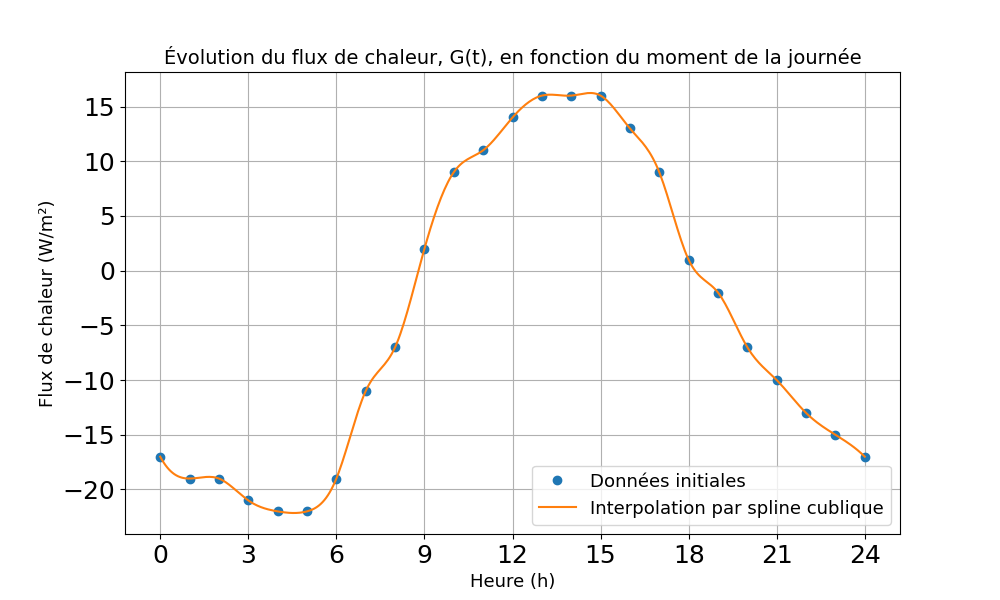
\includegraphics[width=0.70
            \linewidth]{Rapport/figures/PerteEtGain.png}
            \caption{Allure de la fonction $G(t)$}
            \label{fig:PerteEtGain}
        \end{figure}
        Nous remarquons que le fonction a bien interpolée car elle coïncide avec tous les points expérimentaux fournis dans \texttt{PerteEtGain.txt}.
        
\section{Mise en place de la modélisation}
    \subsection{Encodage de \texttt{odefunction}}
        L'énonce impose qu'\texttt{odefunction} reçoive en arguments les températures en $\degree C$, il faut donc incrémenter chaque température de $273,15\degree C$ pour passer de degré Celsius à Kelvin, ce qui est logique car les équations, traitées par la suite, sont exprimées en Kelvin. La fonction consiste à définir le système d'équations différentielles ordinaires 
        \begin{equation}
           C_{cc} \frac{dT_{cc}}{dt} = -\frac{1}{R_{cc-c1}} (T_{cc} - T_{c1}) - \frac{1}{R_{x}} (T_{cc} - T_{t}) + \frac{1}{R_{c2-cc}} (T_{c2} - T_{cc})
            \label{eq:Tcc}
        \end{equation}
        \begin{equation}
            C_{c1} \frac{dT_{c1}}{dt} = -\frac{1}{R_{cc-c1}} (T_{c1} - T_{cc})
            \label{eq:Tc1}
        \end{equation}
        \begin{equation}
            C_{c2} \frac{dT_{c2}}{dt} = -\frac{1}{R_{c2-cc}}(T_{c2} - T_{cc}) + \frac{1}{R_{r-s} + R_{s-c2}}(T_{room} - T_{c2})
            \label{eq:Tc2}
        \end{equation}
        \begin{equation}
            C_{room} \frac{dT_{room}}{dt} = -\frac{1}{R_{r-s} + R_{s-c2}} (T_{room} - T_{c2}) + G(t)
            \label{eq:Troom}
        \end{equation}
        \begin{equation}
            C_w \frac{dT_t}{dt} = -\frac{1}{R_x} (T_t - T_{cc}) - \frac{1}{R_w} (T_t - T_w)
            \label{eq:Tt}
        \end{equation}
        où T, R et C représentent respectivement la température ($K$),la résistance thermique ($m²K/W$) et la capacité thermique spécifique ($kJ/m²K$). \\
        
        
        Il faut ensuite traiter les différentes valeurs que peut prendre la température de l'eau sein des tubes, $T_w$. Il faut modifier sa valeur en fonction de la valeur courante du temps \texttt{t}.
        Dans le cas du scénario 1, on a
        \begin{itemize}
            \item Si $\texttt{t} \in [0,4]$ :
            $T_w = 18\degree C = 291,15 K$
            \item i $\texttt{t} \in \: ]4, 24]$: Le dernier terme de l'équation \ref{eq:Tt} peut être rejeté.
        \end{itemize}
        Les dérivées des température à retourner doivent être multiplier par $3600$ afin de passer de $K/s$ à $K/h$.
        
    \subsection{Méthode d'Euler}

        La méthode d’Euler explicite est une méthode numérique simple d’approximation des solutions d’équations différentielles ordinaires. L’approximation repose sur le processus itératif suivant suivant :
        \begin{equation}
                    T_{i+1} = T_i + h\cdot f(t_i, T_i)
        \end{equation}
        où $f(t_i, T_i)$ représente \texttt{odefunction(t[i], T[i])} et $h$ est le pas.
        Les paramètres de la fonction sont
        \begin{itemize}
            \item \texttt{[t0,tf]} : l'intervalle de temps sur lequel résoudre le système d'équations différentielles ordinaires,
            \item \texttt{T0} : les valeurs de température initiales, toutes égales à $15\degree C$,
            \item \texttt{h} : le pas, représentant l'intervalle entre deux points consécutifs dans la discrétisation du temps.
        \end{itemize}
        
    \subsection{Méthode Runge-Kutta d'ordre 4/5}

        La méthode de Runge-Kutta d'ordre 4/5, aussi appelé RK45, utilisée par la fonction \texttt{solve\_ivp} de la sous-bibliothèque \texttt{integrate} de \texttt{scipy}, permet une plus grande précision qu'Euler car elle ajuste dynamiquement le pas pour optimiser la précision de la solution.
        Les paramètres de la fonction sont
        \begin{itemize}
            \item \texttt{[t0,tf]} : l'intervalle de temps sur lequel résoudre le système d'EDO,
            \item \texttt{T0} : les valeurs de température initiales, toutes égales à $15\degree C$,
            \item \texttt{rtol} : la tolérance relative du solveur, \texttt{solve\_ivp}.
        \end{itemize}

        Les deux méthodes sont valables et aboutissent, en principe, aux mêmes résultats numériques, comme en témoigne la figure \ref{fig:Comparaison}.
        
        \begin{figure}
            \centering
            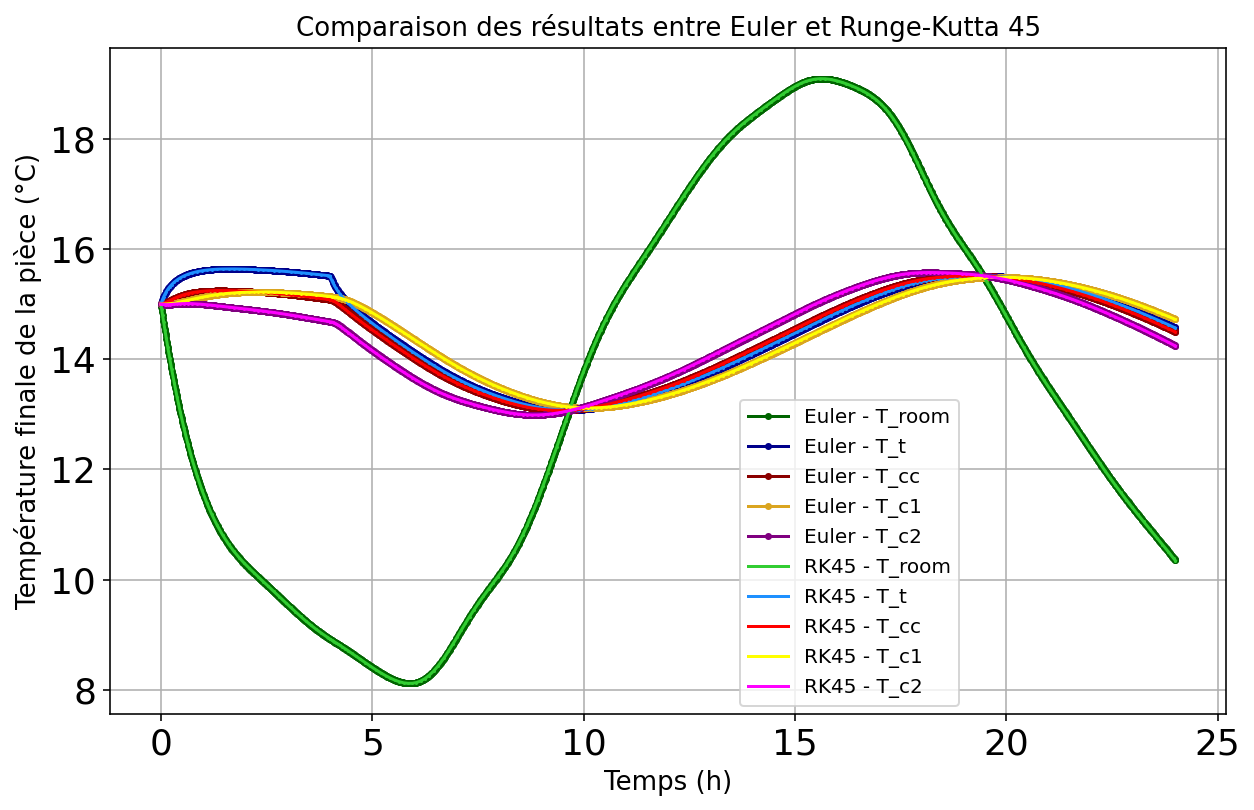
\includegraphics[width=0.70\linewidth]{Rapport/figures/ComparaisonEulerRK45.png}
            \caption{Comparaison des températures entre Euler et Runge-Kutta 45}
            \label{fig:Comparaison}
        \end{figure}

        En somme, la méthode d'Euler est plus rapide mais peut manquer de précision car cette dernière dépend du pas $h$. Tandis que \texttt{solve\_ivp} est plus précis mais plus coûteux. Privilégier une ou l'autre méthode dépend des besoins du programmeur : précision ou économie de ressources.
        
    \subsection{Convergence d'Euler en fonction de $h$}
        Une analyse de l'erreur en fonction du pas de temps $h$ a été réalisée en comparant la solution obtenue avec Euler à une solution de référence avec \texttt{solve\_ivp}. Pour ce faire, la solution de référence a été interpolée sur les pas d'Euler. Ensuite, l'erreur absolue moyenne pour chaque pas candidat $h_{test}$ a été évaluée comme la moyenne de $\left|T_{Euler}-T_{r\Acute{e}f}\right|$. Celle-ci peut être représentée sur la figure \ref{fig:Optimal}.
        \begin{figure}
            \centering
            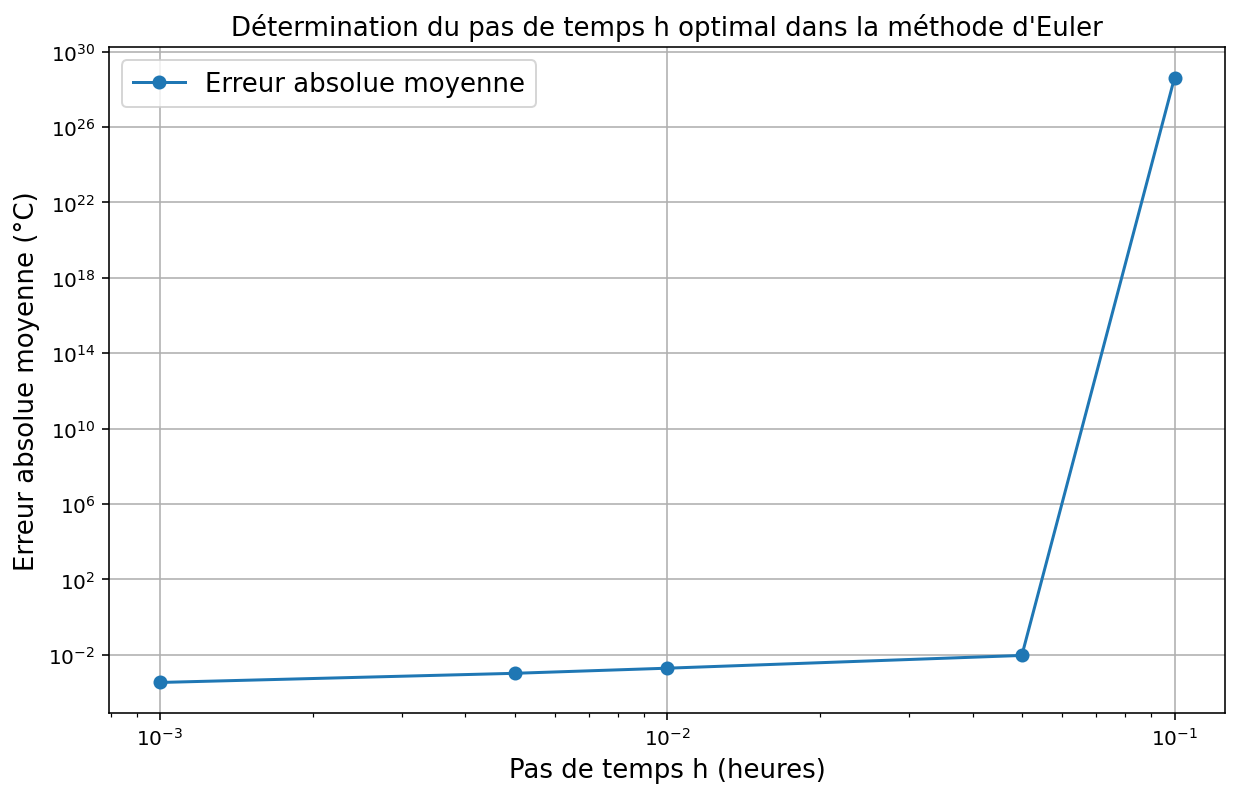
\includegraphics[width=0.70\linewidth]{Rapport/figures/PasEulerOptimal.png}
            \caption{Détermination de l'erreur moyenne de la méthode d'Euler}
            \label{fig:Optimal}
        \end{figure}
        Remarquons que l'erreur diminue lorsque $h$ diminue, ce qui est cohérent car si le pas diminue, la résolution est d'autant plus précise. De plus, la fonction tracée est linéaire lorsqu'on trace le graphe sur une échelle logarithmique. Cela s'explique par le fait que la méthode d'Euler possède un ordre de convergence égal à 1, ce qui implique une erreur en $O(h)$. Il vient alors de faire un compromis et choisir $h=10^{-2}$ qui est plus précis que $h=10^{-1}$ et plus rapide que $h=10^{-3}$.

    \subsection{État stationnaire}\label{section:EtatStationnaire}
        Pour calculer l'évolution des températures jusqu'à atteindre la critère d'arrêt, signe d'état stationnaire,
        \begin{equation}
            T_{room}(t_f) - T_{room}(t_f - 24) < 0.01\degree C
        \end{equation}
        il suffit de de résoudre le système d'équations différentielles ordinaires pour 24 heures, en boucle, en remplaçant les températures initiales par les températures finales calculées après chaque fin de journée, jusqu'à satisfaire le critère d'arrêt et donc atteindre l'état stationnaire du système. Le graphe traçant l’évolution des températures de la pièce et de la partie inférieure du béton en fonction du temps jusqu’à l’état stationnaire est illustré à la figure \ref{fig:convergence}.
        \begin{figure}
            \centering
            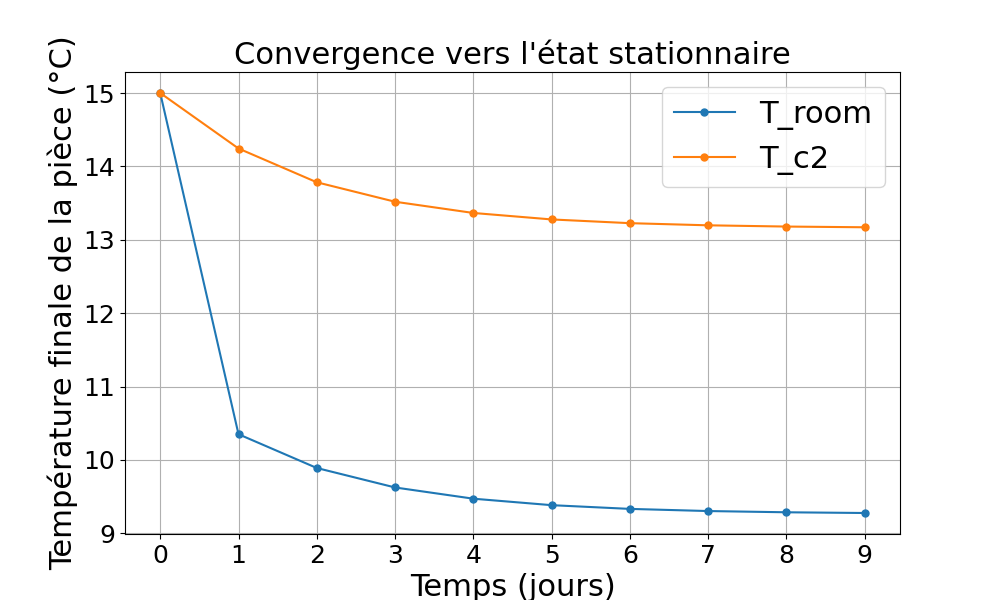
\includegraphics[width=0.70\linewidth]{Rapport/figures/Convergence.png}
            \caption{Convergence vers l'état stationnaire des températures de la pièce et de la partie inférieure du béton.}
            \label{fig:convergence}
        \end{figure}
        Remarquons que la température de la pièce converge vers une valeur beaucoup plus faible que celle du béton. Ceci, s'explique par l'influence des flux de chaleur $G(t)$, baissant la température de la pièce tout au long de la journée.

    \subsection{Comparer les scénarios}
        Pour les calculs il suffit de reprendre la démarche de la question \ref{section:EtatStationnaire}, il faut adapter \texttt{odefunction} aux scénarios 2 et 3. \begin{itemize}
            \item Scénario 2 : 
                    \begin{itemize}
                        \item Si $\texttt{t} \in [0,4]$: $T_w = 18\degree C = 291,15 K$,
                        \item Si $\texttt{t} \in \: ]4,13]$: $T_w = 28\degree C = 301,15 K$,
                        \item Si $\texttt{t} \in \: ]13, 24]$: Le dernier terme de l'équation \ref{eq:Tt} peut être rejeté.

                    \end{itemize}
            \item Scénario 3 : 
                    \begin{itemize}
                        \item Si $\texttt{t} \in [0,12]$: $T_w$ = $28\degree C = 301,15 K$,
                        \item Si $\texttt{t} \in \: ]12,24]$: $T_w$ = $18\degree C = 291,15 K$.

                    \end{itemize}
        \end{itemize}

        On obtient ainsi les résultats, pour chaque température, illustrés sur les figures \ref{fig:Scenario},
        \begin{figure}
            \centering
            
            \begin{subfigure}{0.48\textwidth}
                \centering
                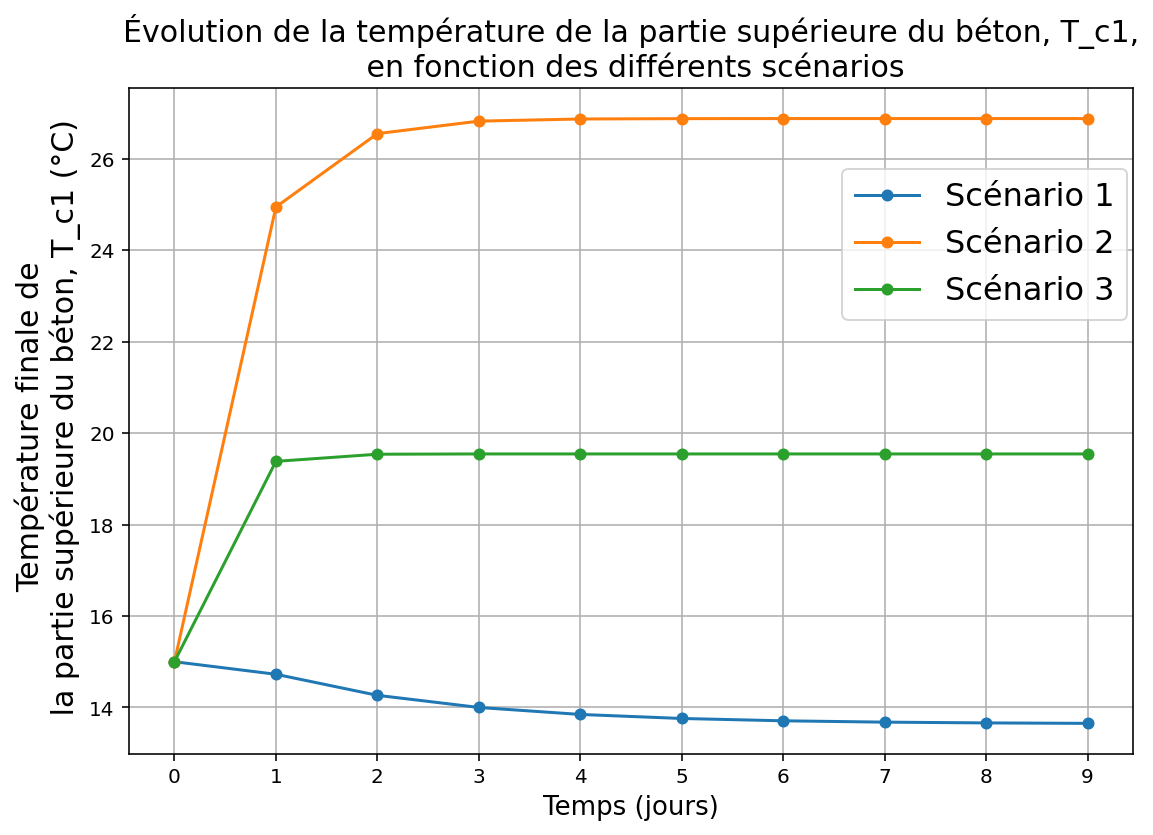
\includegraphics[width=1\linewidth]{Rapport/figures/T_c1.png}
                \caption{Partie supérieure du béton} 
                \label{fig:Tc1}
            \end{subfigure}
            \hfill
            \begin{subfigure}{0.48\textwidth}
                \centering
                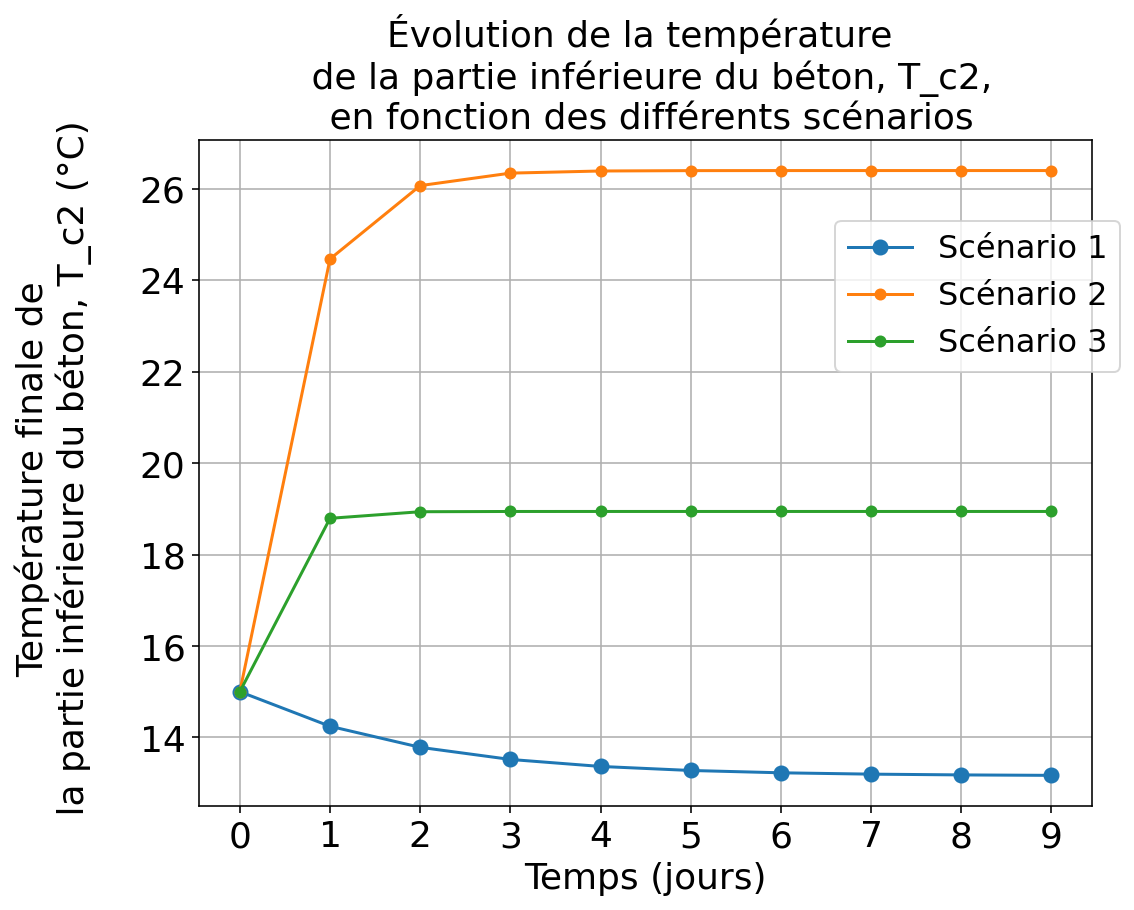
\includegraphics[width=1\linewidth]{Rapport/figures/T_c2.png}
                \caption{Partie inférieur du béton} 
                \label{fig:Tc2}
            \end{subfigure}
            \begin{subfigure}{0.48\textwidth}
                \centering
                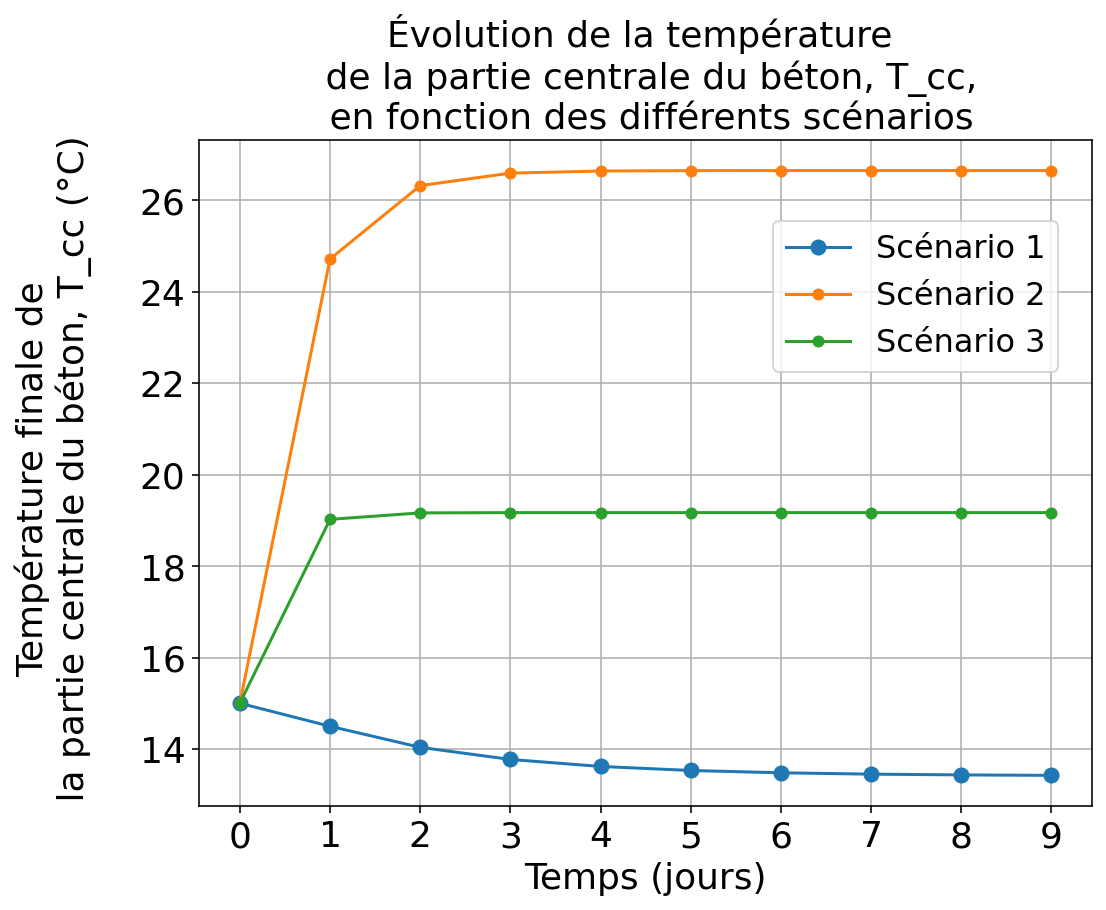
\includegraphics[width=1\linewidth]{Rapport/figures/T_cc.png}
                \caption{Partie centrale du béton} 
                \label{fig:Tcc}
            \end{subfigure}
            
            \begin{subfigure}{0.48\textwidth}
                \centering
                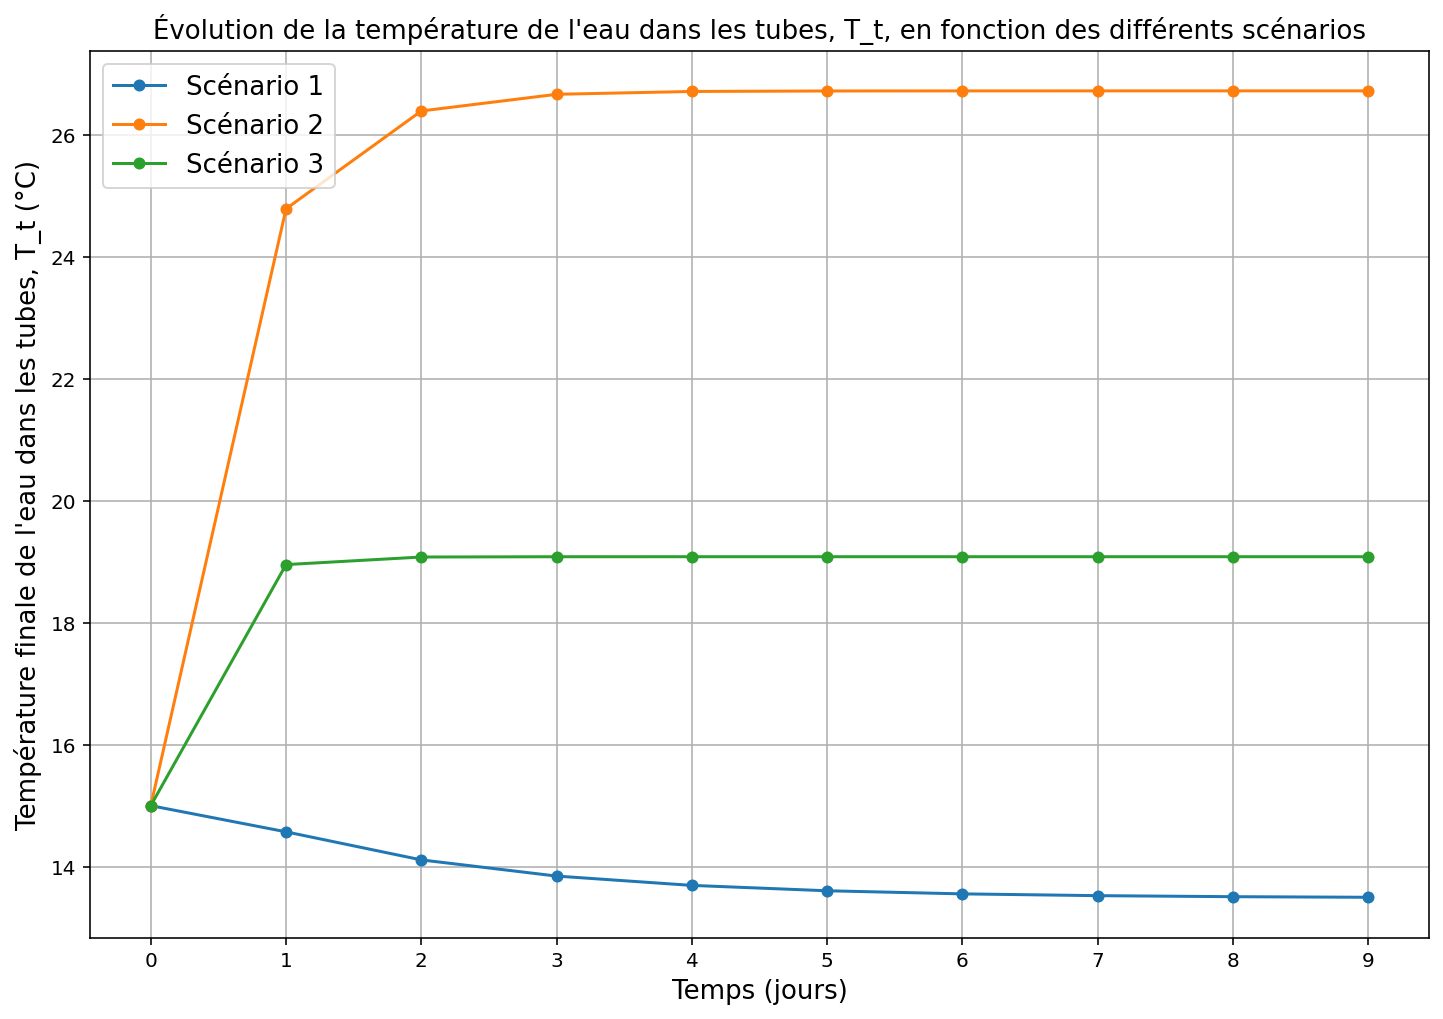
\includegraphics[width=1\linewidth]{Rapport/figures/T_t.png}
                \caption{Tubes} 
                \label{fig:Tt}
            \end{subfigure}
            \begin{subfigure}{0.48\textwidth}
                \centering
                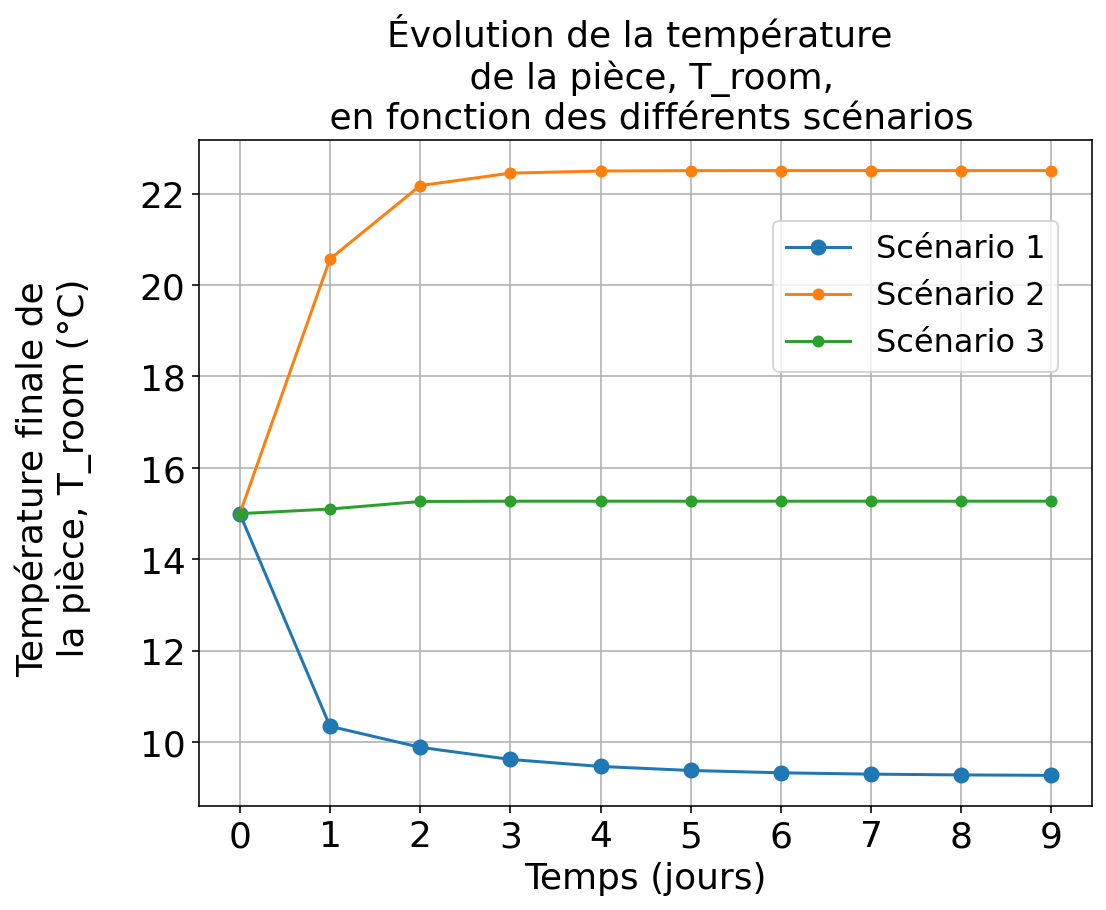
\includegraphics[width=1\linewidth]{Rapport/figures/T_room.png}
                \caption{Pièce} 
                \label{fig:Troom}
            \end{subfigure}
            
            \caption{Évolution des températures suivant les différents scénarios}
            \label{fig:Scenario}
        \end{figure}

        Comme souligné précédemment, la température de la pièce est la seule à présenter une différence notable dans sa variation temporelle comparée à toutes les autres.

\section{Régulation automatisée du bâtiment}

    \subsection{Détermination de $T_{max}$}
    
        Il suffit d'adapter \texttt{odefunction} en fonction de $\Delta t$ et à l'aide de la fonction \texttt{max} et \texttt{argmax} de \texttt{numpy}, il est possible de trouver le point culminant de la température de confort, $T_{max}$, définit selon
        \begin{equation}
            T_{max} = \max \left( T_{confort}(t, \Delta t) \right)
        \end{equation}
        et d'en imposer une valeur maximale. Cette fonction a permis le dessin de la figure \ref{fig:24h} qui trouve la température de confort maximale pour un $\Delta t = 1 $ fixé arbitrairement.
        \begin{figure}
            \centering
            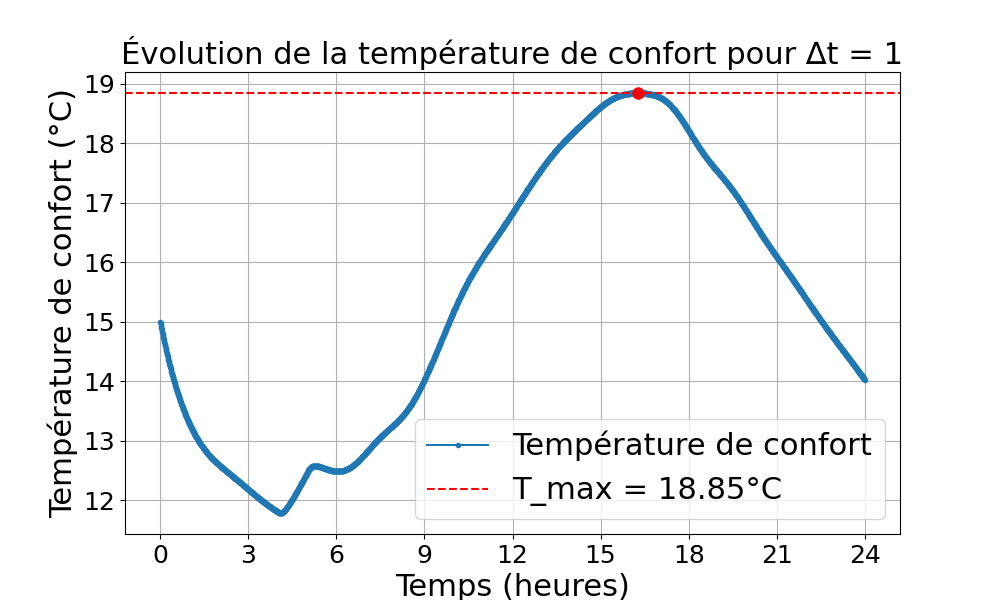
\includegraphics[width=0.70\linewidth]{Rapport/figures/T_confort_24h.png}
            \caption{Détermination de la température max lors des premières 24h avec $\Delta t = 1$}
            \label{fig:24h}
        \end{figure}
    
    \subsection{Détermination de $\Delta t_{optimal}$}\label{section:Delta_t_optimal}

        Par définition de $\Delta t_{optimal}$, on a
        \begin{equation}
            \Delta t_{optimal} = \arg \max_{\Delta t} \left(T_{confort}(t, \Delta t) \right)
        \end{equation}
        de sorte que
        \begin{equation}
            T_{max}^d = T_{max}(\Delta t_{optimal}) = \max_{\Delta t} \left( T_{max}(\Delta t) \right)
        \end{equation}
        La recherche revient donc à trouver la racine de la fonction $f(\Delta t)$ définit comme
        \begin{equation}
            f(\Delta t) = T_{max}(\Delta t) - T_{max}^d
        \end{equation}
        La méthode de la sécante semble adéquate pour cette tâche car elle converge rapidement et fournit un résultat plus précis que la bissection. Il vient ensuite de choisir l'intervalle compris entre 0.1 et 8 heures. La vérification de cet intervalle repose sur le théorème des valeurs intermédiaires. En effet, La condition $f(0.1)\cdot f(8.0) < 0$ garantit l'existence d'une racine dans l'intervalle choisi, confirmant ainsi la pertinence de ces bornes.
        Concernant la tolérance, une précision de $\pm 0.01$ h sur $\Delta t$ est suffisante, car elle induit une variation négligeable de la température maximale $T_{\max}$. Un compromis entre coût de calcul et précision a été adopté : une tolérance plus stricte, par exemple $10^{-5}$, augmenterait significativement le temps de calcul sans apporter de bénéfice pratique notable. La détermination de ce $\Delta t_{optimal}$ est représenté à la figure \ref{fig:T_confort_optimal}.
        \begin{figure}
            \centering
            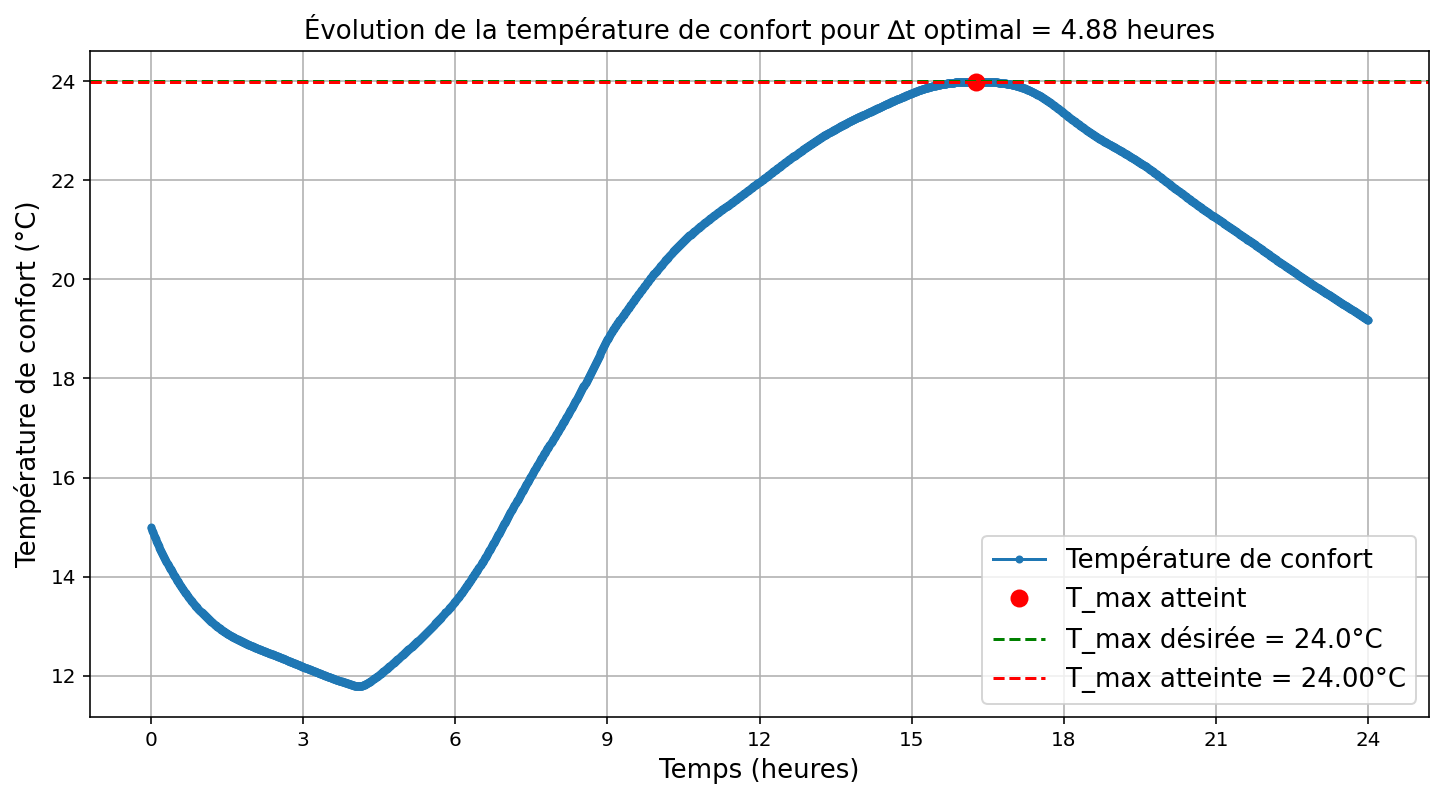
\includegraphics[width=0.70\textwidth]{Rapport/figures/T_confort_optimal.png}
            \caption{Évolution de la température de confort avec $\Delta t_{optimal} = 2.46h$ et $T_{max}^d = 21$\degree C}
            \label{fig:T_confort_optimal}
        \end{figure}
        
    \section{Question 4.3}
        
         Il vient de refaire la même chose qu'à la question \ref{section:Delta_t_optimal} mais lorsque le système est à l'état stationnaire. Ainsi, il vient de réutiliser l'implémentation de la question \ref{section:EtatStationnaire}. Il se trouve que celui-ci se stabilise après 8 jours, comme le montre la figure \ref{fig:T_Confort_convergence}.
         \begin{figure}
             \centering
             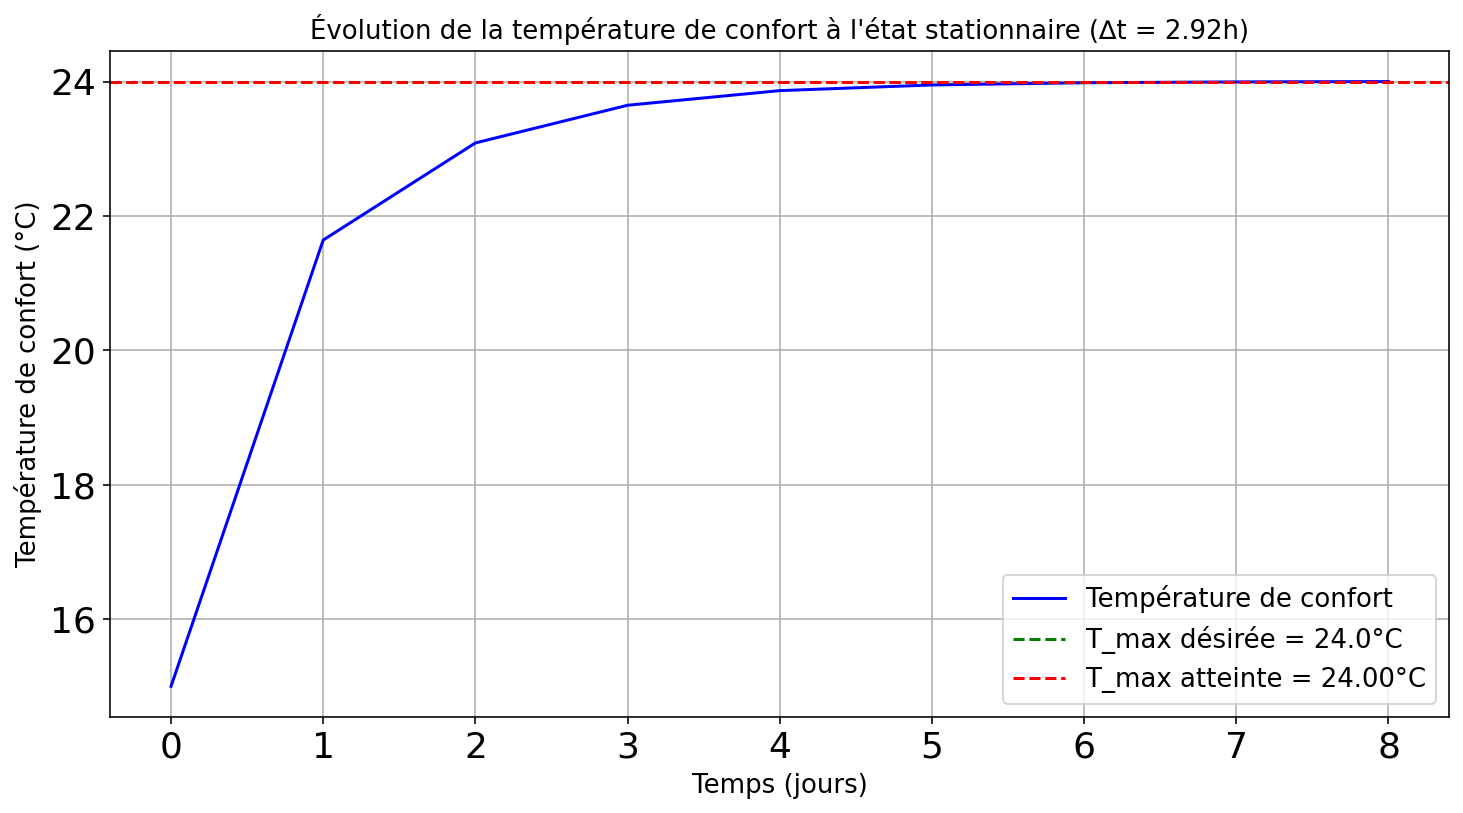
\includegraphics[width=0.48\linewidth]{Rapport/figures/ConvergenceT_confort.png}
             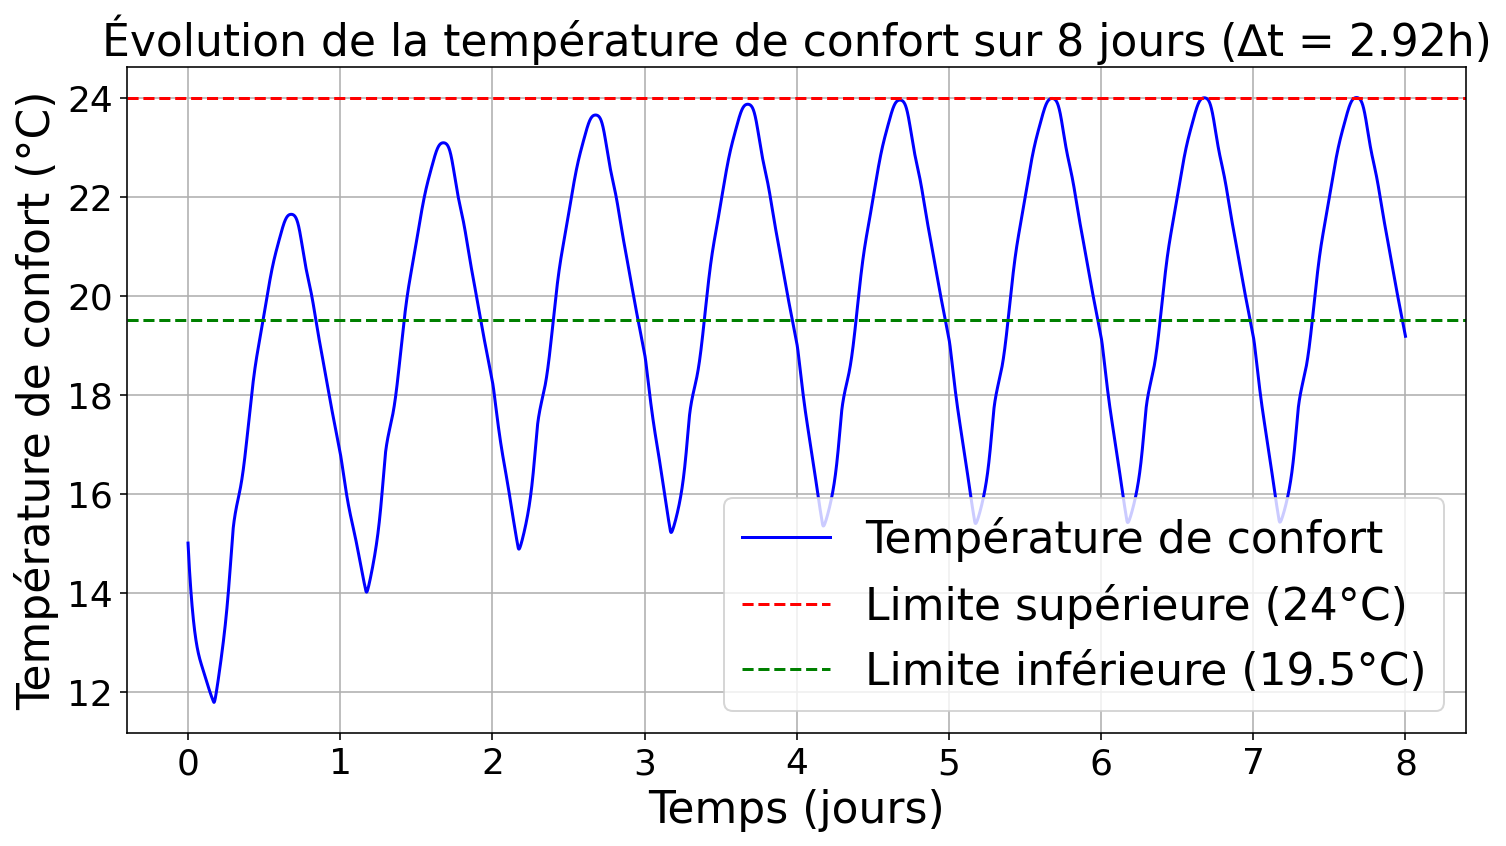
\includegraphics[width=0.48\linewidth]{Rapport/figures/T_confort_8jours.png}
             \caption{Caption}
             \label{fig:enter-label}
         \end{figure}
    
            



%\newpage
%\bibliography{mybib}


\end{document}
%%% Local Variables: 
%%% mode: latex
%%% TeX-master: t
%%% End: 
